\section{Incremento 1}
Este primer incremento se centra en la configuración del proyecto y implementación de registro, autenticación y perfil de usuario.

\subsection{Análisis}
Con respecto a la \textbf{configuración del proyecto}, se ha decidido utilizar la plataforma backend \emph{Supabase} y los frameworks \emph{Next.js} para el desarrollo de la aplicacion web y \textit{Tailwind CSS} para el manejo de estilos. Como punto de partida, se ha utilizado la plantilla \emph{Next.js Supabase Auth Starter} \cite{nextjs_supabase_starter}, la cual incluye la configuración básica para el registro y autenticación de usuarios mediante \emph{Supabase}.

Por otro lado, en cuanto a la \textbf{implementación de registro, autenticación y perfil de usuario}, se han desarrollado los requisitos funcionales y no funcionales definidos en \tabref{tab:requisitosfuncionalesincremento1} y no funcionales \tabref{tab:requisitosnofuncionales}.

\begin{table}[H]
    \centering
    \scriptsize
    \begin{tabular}{l p{0.58\textwidth} p{0.20\textwidth} l}
        \textbf{ID} & \textbf{Requisito Funcional} & \textbf{Funcionalidad} & \textbf{Prioridad} \\ \hline
        RF1  & El usuario debe poder iniciar y cerrar sesión. & Cuenta de usuario & Alta \\ \hline
        RF2  & El usuario debe poder registrarse utilizando su correo electrónico, contraseña y un nombre de usuario. & Cuenta de usuario & Alta \\ \hline
        RF3  & El usuario debe poder modificar su perfil. & Cuenta de usuario & Alta \\ \hline
        RF4  & El usuario debe poder recuperar o restablecer su contraseña en caso de olvido. & Cuenta de usuario & Alta \\ \hline
    \end{tabular}
    \caption{Requisitos Funcionales desarrollados en el incremento 1}\label{tab:requisitosfuncionalesincremento1}
\end{table}

\begin{table}[H]
    \centering
    \scriptsize
    \begin{tabular}{l p{0.79\textwidth} l}
    \textbf{ID} & \textbf{Requisito No Funcional} & \textbf{Prioridad} \\ \hline
    RNF1 & El sistema debe ser responsivo, adaptándose a diferentes tamaños de pantalla y dispositivos. & Alta \\ \hline
    RNF2 & El sistema debe incluir una descripción textual (alt) en todas las imágenes. & Alta \\ \hline
    RNF3 & El sistema debe incluir un aria-label o aria-labelledby en todos los elementos interactivos, describiendo su función para lectores de pantalla. & Alta \\ \hline
    RNF4 & El sistema debe proporcionar navegación mediante un encabezado (header) y un pie de página (footer) consistentes en todas las vistas. & Alta \\
    \end{tabular}
    \caption{Requisitos No Funcionales desarrollados en el incremento 2}\label{tab:requisitosnofuncionales}
\end{table}

\subsection{Diseño de datos}
La estructura de datos inicial se basa en la tabla de usuarios predeterminada de \emph{Supabase}, la cual incluye los campos mínimos necesarios para la autenticación de usuarios (destacamos id, email, contraseñas y fecha de creación). Por otro lado, se ha añadido una tabla adicional denominada \emph{profiles} para almacenar información adicional de los usuarios (para este primer incremento solo se ha incluido el nombre de usuario y fecha de creación). Las tablas de \emph{usuarios} y \emph{profiles} están directamente relacionadas entre sí, tal y como podemos observar en \figref{fig:diagrama_datos_i1}.

\begin{figure}[H]
    \centering
    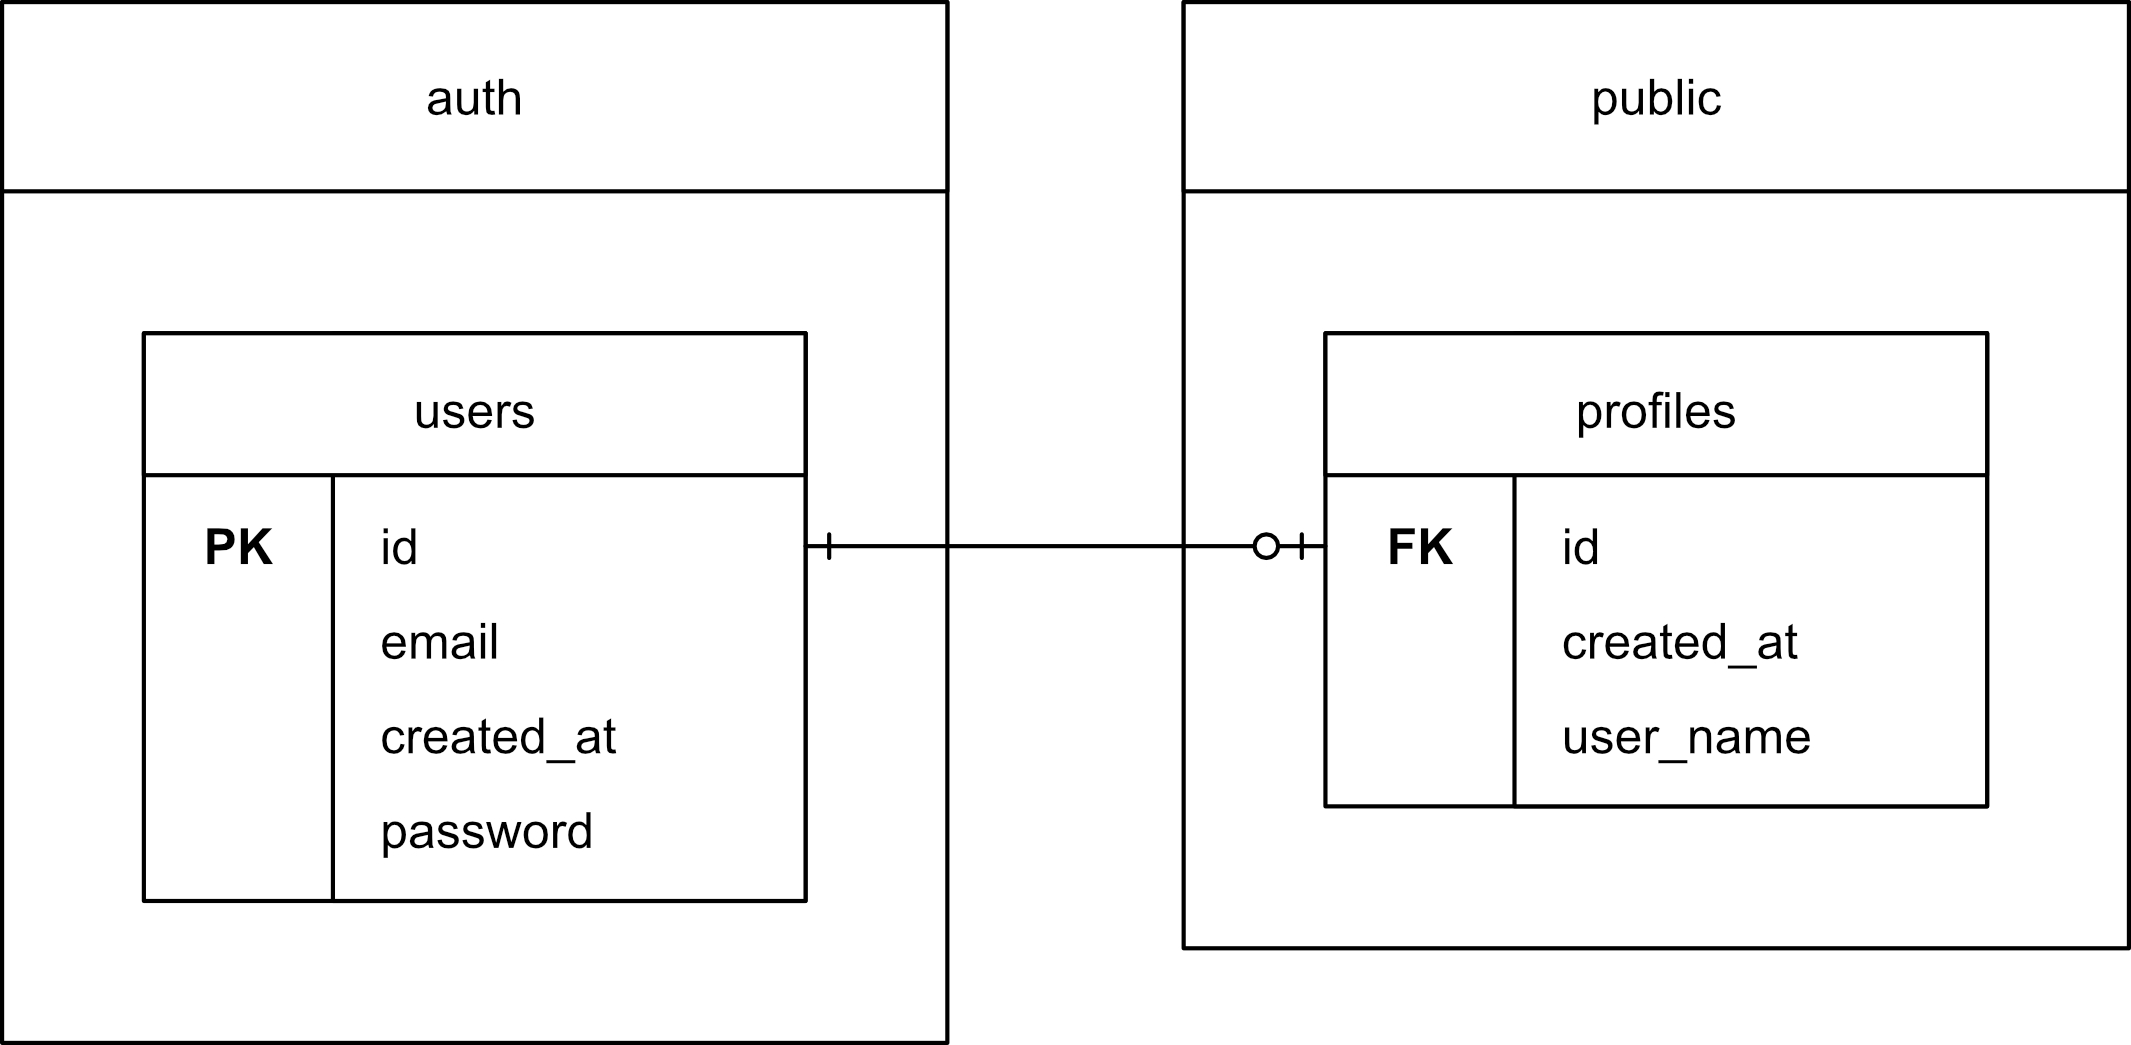
\includegraphics[width=0.8\textwidth]{Ilustraciones/desarrollo/incremento1/diagrama_datos_i1.jpg}
    \caption{Diagrama de estructura de datos de los perfiles de usuario}\label{fig:diagrama_datos_i1}
\end{figure}

\subsection{Diseño de interfaz}
Al tratarse del primer incremento, fué de vital importancia comenzar a definir la guía de diseño de la interfaz. En primer lugar, se estableció una paleta de colores con tonalidades de grises y azules \figref{fig:ui_palette}. Seguidamente se definió la guía de colores \figref{fig:ui_guide}, estableciendo los colores según su función (fondos, textos, primarios, etc.), con sus respectivos colores principales y de primer plano.

\begin{figure}[H]
    \centering
    \begin{subfigure}[t]{0.48\textwidth}
        \centering
        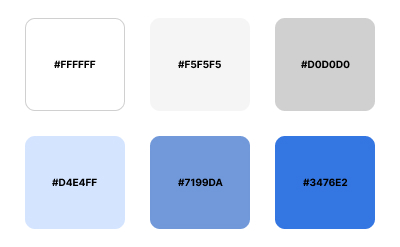
\includegraphics[width=1\textwidth]{Ilustraciones/desarrollo/incremento1/diseño/color_palette.jpg}
        \caption{Paleta de colores}\label{fig:ui_palette}
    \end{subfigure}
    \hfill
    \begin{subfigure}[t]{0.48\textwidth}
        \centering
        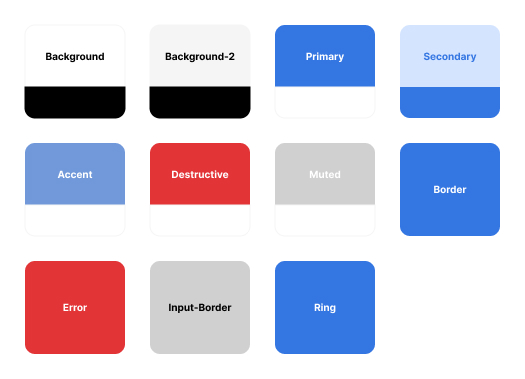
\includegraphics[width=\textwidth]{Ilustraciones/desarrollo/incremento1/diseño/color_scheme.jpg}
        \caption{Guía de colores. Arriba principal, abajo primer plano.}\label{fig:ui_guide}
    \end{subfigure}\caption{Colores utilizados en la interfaz}\label{fig:ui_colors}
\end{figure}

En segundo lugar, se diseñó el isologo de la aplicación web \figref{fig:ui_logo}, el cual combina el timple con el nombre de la aplicación web \emph{Timple Tabs}.

\begin{figure}[H]
    \centering
    
\includegraphics[width=0.5\textwidth]{Ilustraciones/desarrollo/incremento1/diseño/logo_2.png}
    \caption{Isologo de la aplicación web}\label{fig:ui_logo}
\end{figure}

En tercer lugar, se diseñaron algunos de los elementos comunes de la interfaz de usuario. Para este primer incremento fué fundamental el diseño de botones \figref{fig:ui_buttons} y campos de formulario \figref{fig:ui_fields}, en los que se hace uso de los iconos de la biblioteca pública \emph{Lucide Icons} \cite{lucide_icons}.

\begin{figure}[H]
    \centering
    \begin{subfigure}[t]{0.48\textwidth}
        \centering
        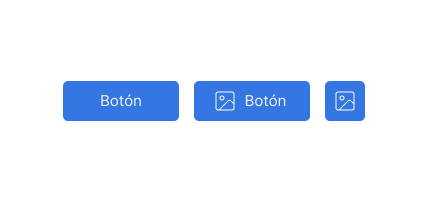
\includegraphics[width=1\textwidth]{Ilustraciones/desarrollo/incremento1/diseño/buttons.jpg}
        \caption{Botones y sus variantes según espacio}\label{fig:ui_buttons_variants}
    \end{subfigure}
    \hfill
    \begin{subfigure}[t]{0.48\textwidth}
        \centering
        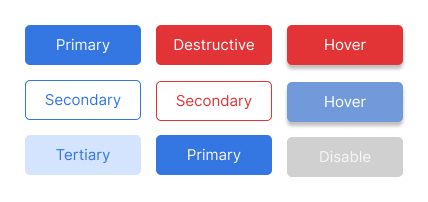
\includegraphics[width=1\textwidth]{Ilustraciones/desarrollo/incremento1/diseño/button_color_scheme.jpg}
        \caption{Botones y sus variantes según función y estado}\label{fig:ui_buttons_color}
    \end{subfigure}
    \vspace{1em}
    \begin{subfigure}[t]{\textwidth}{
        \centering
        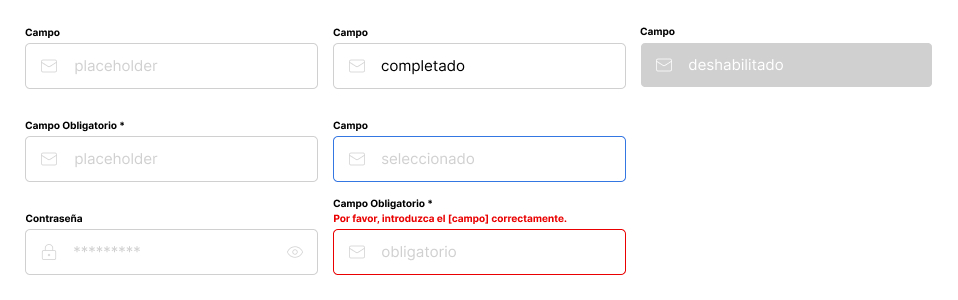
\includegraphics[width=\textwidth]{Ilustraciones/desarrollo/incremento1/diseño/fields.jpg}
        \caption{Campos y sus variantes según función y estado}\label{fig:ui_fields}}    
    \end{subfigure}
    \caption{Diseño de elementos comunes}\label{fig:ui_buttons}
\end{figure}

Finalmente, con todos los elementos mencionados anteriormente, se definió una básica guía de diseño que sirvió como referencia para el diseño de las pantallas correspondientes al registro, inicio de sesión \figref{fig:ui_login}, recuperación de contraseña \figref{fig:passrec} y registro \figref{fig:ui_register}. 

\begin{figure}[H]
    \centering
    \begin{subfigure}[t]{0.3\textwidth}
        \centering
        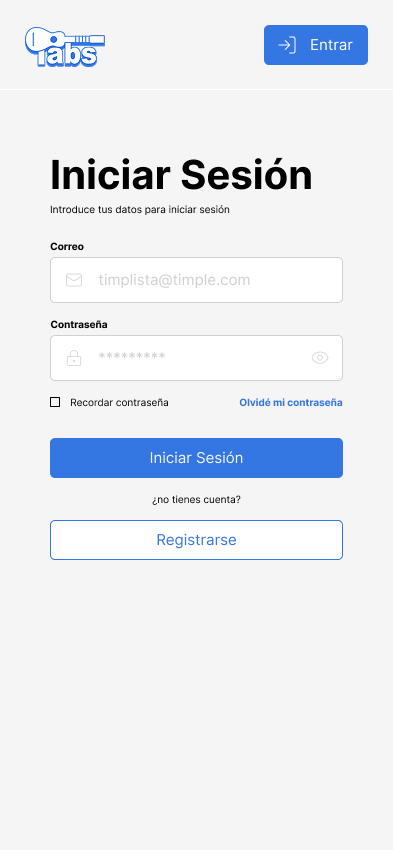
\includegraphics[width=0.8\textwidth]{Ilustraciones/desarrollo/incremento1/diseño/login.jpg}
        \caption{Diseño de página de inicio de sesión}\label{fig:ui_login}
    \end{subfigure}
    \hfill
    \begin{subfigure}[t]{0.3\textwidth}
        \centering
        
\includegraphics[width=0.8\textwidth]{Ilustraciones/desarrollo/incremento1/diseño/password_recovery.jpg}
        \caption{Diseño de página de recuperación de contraseña}\label{fig:passrec}
    \end{subfigure}
    \hfill
    \begin{subfigure}[t]{0.30\textwidth}
        \centering
        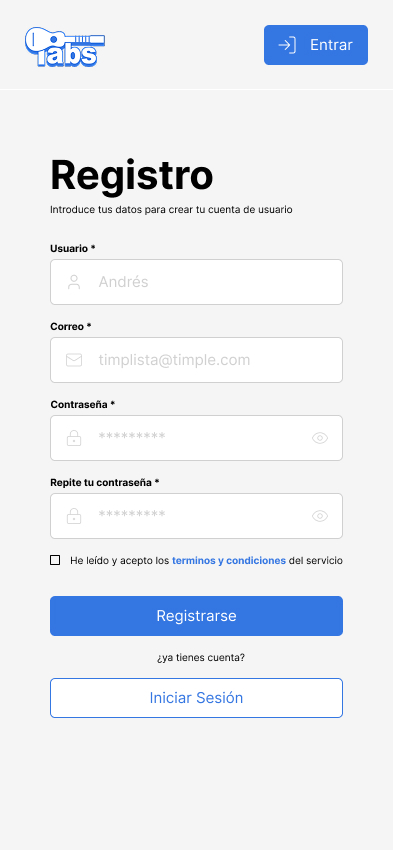
\includegraphics[width=0.8\textwidth]{Ilustraciones/desarrollo/incremento1/diseño/register.jpg}
        \caption{Diseño de pantalla de registro de usuario con campos vacios}\label{fig:ui_register_empty}
    \end{subfigure}
    \hfill
    \begin{subfigure}[t]{0.30\textwidth}
        \centering
        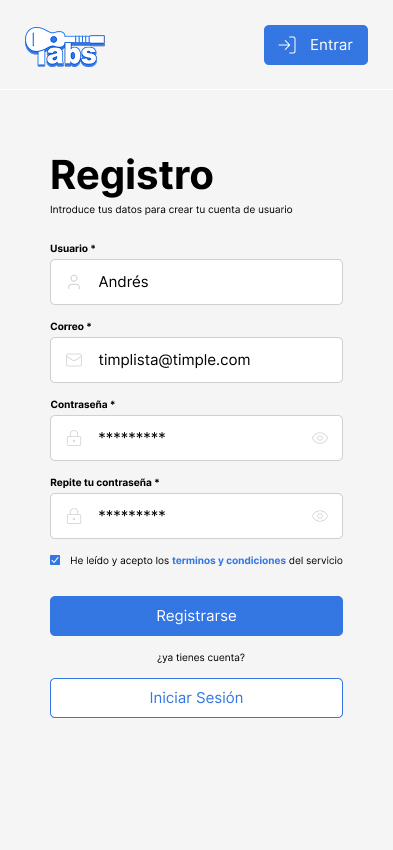
\includegraphics[width=0.8\textwidth]{Ilustraciones/desarrollo/incremento1/diseño/register_filled.jpg}
        \caption{Diseño de pantalla de registro de usuario con campos completados}\label{fig:ui_register_fill}
    \end{subfigure}
    \hfill
    \begin{subfigure}[t]{0.30\textwidth}
        \centering
        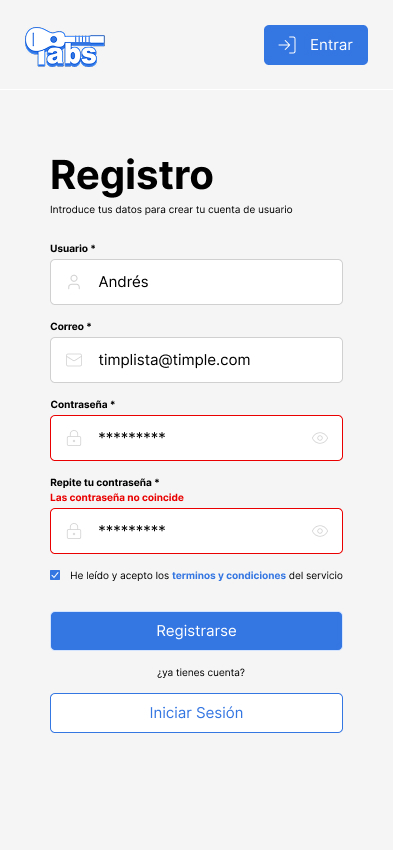
\includegraphics[width=0.8\textwidth]{Ilustraciones/desarrollo/incremento1/diseño/register_error.jpg}
        \caption{Diseño de pantalla de registro de usuario con campos incorrectos}\label{fig:ui_register_fail}
    \end{subfigure}
    \hfill
    \begin{subfigure}[t]{0.3\textwidth}
        \centering
        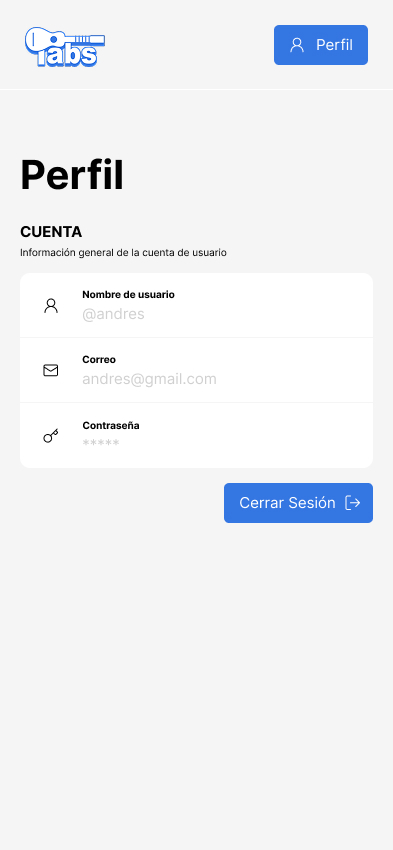
\includegraphics[width=0.8\textwidth]{Ilustraciones/desarrollo/incremento1/diseño/profile.jpg}
        \caption{Diseño de página de perfil de usuario}\label{fig:passrec}
    \end{subfigure}
    \vspace{1em}
    \caption{Diseño de páginas del primer incremento}\label{fig:ui_smt}
\end{figure}

Los anteriores han sido diseñados con el enfoque mobile-first, asegurando una correcta visualización y usabilidad en dispositivos móviles y adaptándose a pantallas de mayor tamaño mediante un diseño responsivo \figref{fig:ui_login_desktop}.

\begin{figure}[H]  
    \centering
    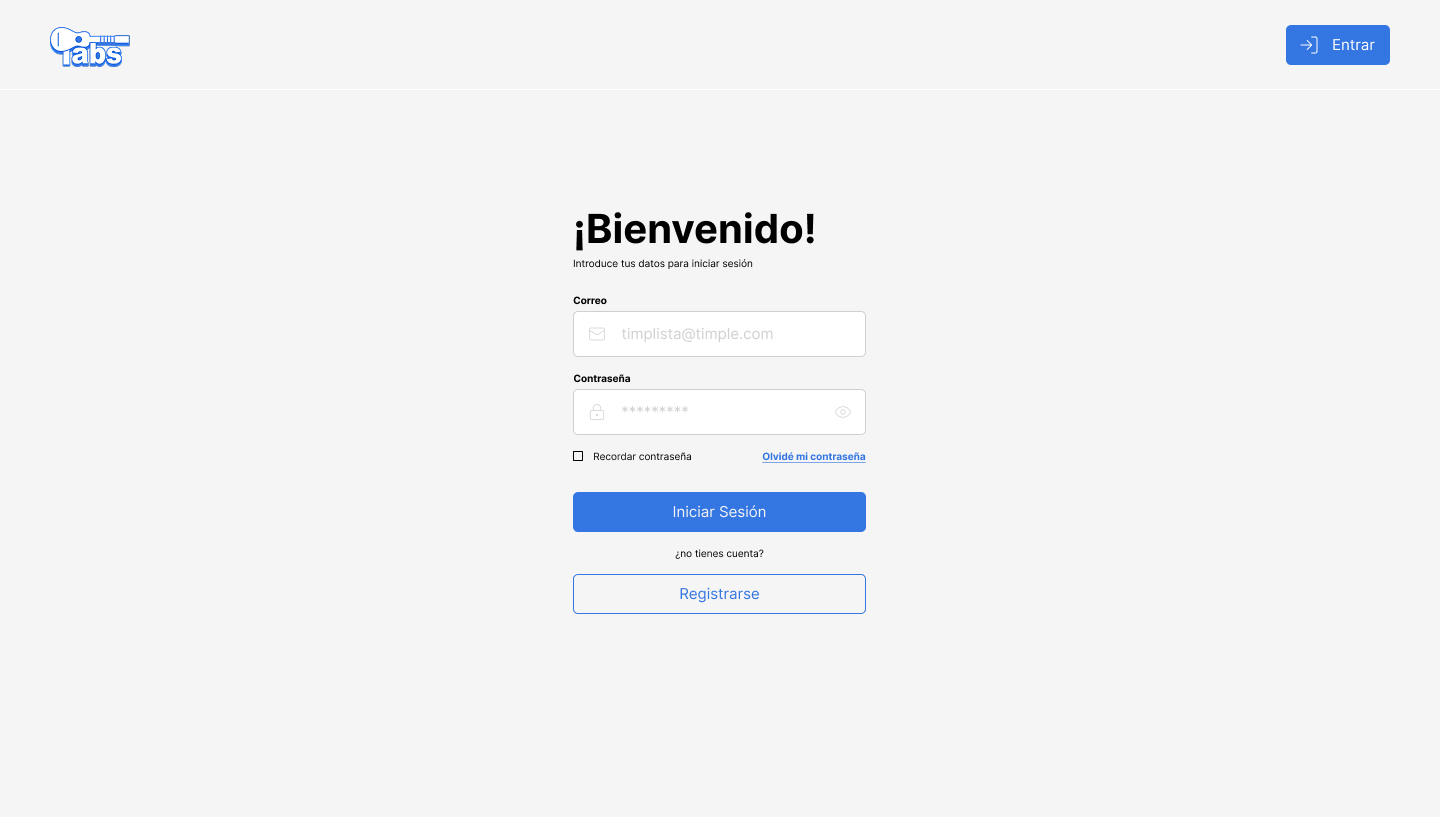
\includegraphics[width=0.8\textwidth]{Ilustraciones/desarrollo/incremento1/diseño/login_big.jpg}
    \caption{Diseño de página de inicio de sesión en pantallas grandes}\label{fig:ui_login_desktop}
\end{figure}